\documentclass[MAIN.tex]{subfiles} 
\begin{document} 
% - http://www.r-bloggers.com/a-startlingly-neat-simple-rule-five-graphs-about-patterns-that-might-surprise-you/
% - http://onlinelibrary.wiley.com/doi/10.1029/1999WR900012/pdf
\begin{frame}
	\begin{figure}
		\centering
		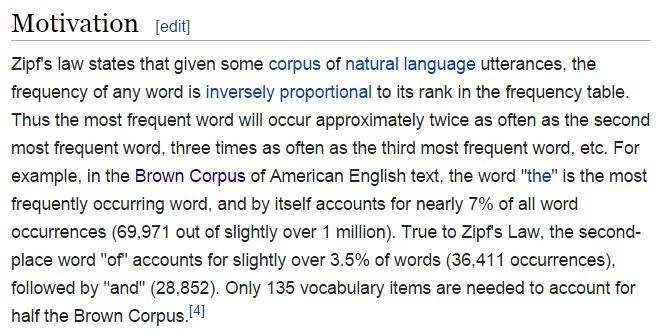
\includegraphics[width=1.01\linewidth]{images/zipfwiki}
	\end{figure}
	
\end{frame}
\begin{frame}
	\begin{figure}
\centering
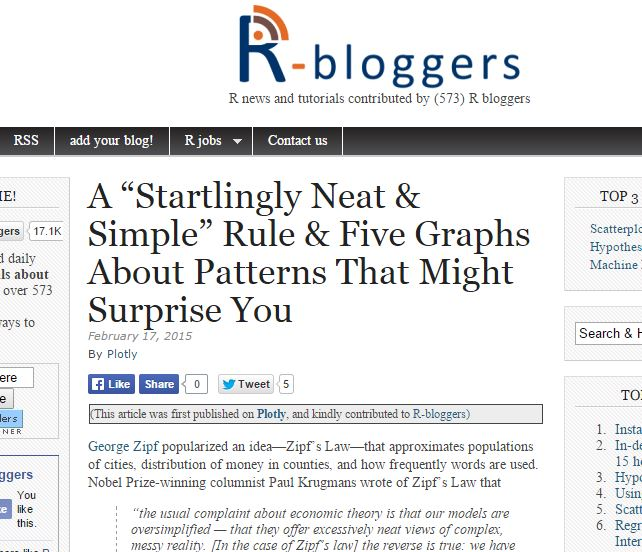
\includegraphics[width=1.01\linewidth]{images/zipf-plotly}
\end{figure}

\end{frame}
\begin{frame}
\frametitle{Zipf Distribution}
\large

George Zipf popularized an idea- ``Zipf’s Law" - that approximates populations of cities, distribution of money in counties, and how frequently words are used.\\ \bigskip Nobel Prize-winning columnist Paul Krugmans wrote of Zipf’s Law that
\begin{quote}
“the usual complaint about economic theory is that our models are oversimplified — that they offer excessively neat views of complex, messy reality. [In the case of Zipf’s law] the reverse is true: we have complex, messy models, yet reality is startlingly neat and simple.”

\end{quote}


\end{frame}
%=====================================================================================%

%\begin{frame}
%\frametitle{Zipf Distribution}
%\begin{itemize}
%\item A Zipfian distribution is a type of power law. A power law occurs when one event varies as a power of another. One application of Zipf’s law states that in texts of natural language (e.g., books), each word is used twice as often as the next most commonly occuring word. 
%\item The graph below applies the rule to word usage in 29 UK books below. “The” occurred 225,300 uses, and was the most commonly used word. \item Note that the graph is interactive; you can press the “play with this data” link to edit, embed, and share your own version. (Plotly Blog page)
%\end{itemize}
%
%\end{frame}
%=====================================================================================%
%
%\begin{frame}
%\frametitle{Zipf Distribution}
%
%Evaluating Power Laws
%
%
%\begin{itemize}
%\item We can test for a power law by plotting frequency (y-axis) against rank (x-axis) on a double log axis. Then check for a straight line.
%\item The graph below shows three attempts to fit a power law function to datasets. The plot on the left is a good fit. The plot in the middle is a decent fit.
%\item  The plot on the right is not a good fit.
%\end{itemize}
% 
%
%\end{frame}
%=====================================================================================%
%
%\begin{frame}
%\frametitle{Zipf Distribution}
%
%
%\textbf{Evaluating Zipfian Distributions For City Populations}
%
%
%
%Another application of Zipf’s law is for populations. 
%We’ve used ggplot2 to graph the population of cities (y-axis) and the rank of each city. 
%In this dataset, New York has the highest population and is ranked first. 
%
%
%\end{frame}
%%=====================================================================================%
%
%\begin{frame}
%\frametitle{Zipf Distribution}
%
%
%
%\textbf{GDP Of Nations}
%
%
%
%We are approaching a Zipfians distribution for country GDP vs rank. 
%
%
%\textbf{Evaluating Power Laws For Many Datasets}
%
%
%
%Researchers use power laws to determine how much inftrasture a city needs, examine the number of gas stations required in a city, and much more. 
%\end{frame}
%=====================================================================================%

%=====================================================================================%
\end{document}